
%Author: Siddhesh Wani
%Date: November 23, 2015








%DO NOT 
%  -- change color scheme
%  -- modify version no.




\documentclass[12pt]{article}
\usepackage{tikz}
\usetikzlibrary{shapes.geometric, arrows}
\usepackage{hyperref}

%DO NOT EDIT start
%Define different shapes to be used in flowchart
\tikzstyle{startstop} = [rectangle, rounded corners, minimum width=3cm, minimum height=1cm,text centered, draw=black, fill=red!30]
\tikzstyle{io} = [trapezium, trapezium left angle=70, trapezium right angle=110, minimum width=3cm, minimum height=1cm, text centered, draw=black, fill=blue!30]
\tikzstyle{process} = [rectangle, minimum width=3cm, minimum height=1cm, text centered, draw=black, fill=orange!30]
\tikzstyle{decision} = [diamond, minimum width=3cm, minimum height=1cm, text centered, draw=black, fill=green!30]
\tikzstyle{arrow} = [thick,->,>=stealth]
%DO NOT EDIT end

\title{Filename.sci}
\author{Siddhesh Wani}
\title{FA_SZ_2.sci}


\begin{document}
\maketitle

\textbf{Introduction}\\
Write some introduction about file here. What input (if any) it accepts, what it does and what is the output (if any).


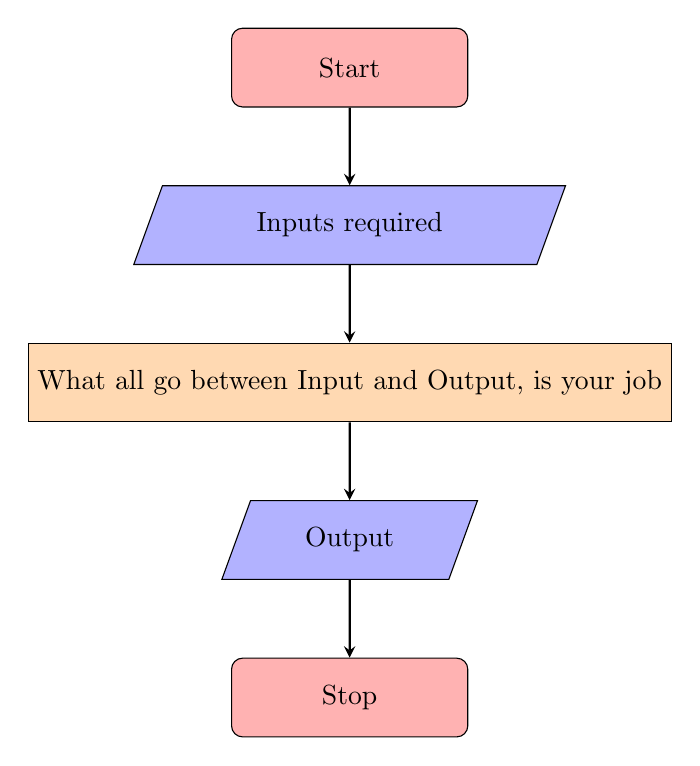
\begin{tikzpicture}[node distance=2cm]
\label{first}
\node (start) [startstop] {Start};
\node (in1) [io, below of=start] {Inputs required };
\node (pro1) [process, below of=in1] {What all go between Input and Output, is your job};
\node (out1) [io, below of=pro1] {Output};
\node (stop) [startstop, below of=out1] {Stop};

\draw [arrow] (start) -- (in1);
\draw [arrow] (in1) -- (pro1);
\draw [arrow] (pro1) -- (out1);
\draw [arrow] (out1) -- (stop);
\end{tikzpicture}


\end{document}